\documentclass[english]{article}
\usepackage{longtable}
\usepackage{amsmath}
\usepackage{ae,aecompl}
\usepackage[T1]{fontenc}
\usepackage[latin9]{inputenc}
\usepackage{textcomp}
\usepackage{graphicx}
\usepackage{eurosym}
\usepackage[hidelinks]{hyperref}
\usepackage{float}
\usepackage{fancyhdr}
\usepackage{tabto}
\usepackage{verbatim}
\usepackage{etoolbox}
\usepackage[table]{xcolor}
\usepackage{booktabs}
\usepackage{wasysym}
\usepackage{multirow}
\usepackage{fancyhdr}
\usepackage{pdflscape}
\usepackage[scaled]{beramono}
\usepackage{csquotes}
\usepackage{comment}
\usepackage{listings}
\usepackage{hhline}


\pagestyle{fancy}
\lhead{\powerenjoy PPD}
\makeatletter
\makeatother
\usepackage{babel}
 \lstset{
 	 breaklines=true,
 	 }
% FP table
\newenvironment{fptable}[2]{
	\begin{center}
	#1
	\begin{longtable}{|c|c|c|c|}
	\hline 
	&
	\multicolumn{3}{|c|}{{#2}}\\\nopagebreak\hline	
}{
	\hline\end{longtable}\end{center}
}

% FP count table
\newenvironment{fpcounttable}[1]{
	\begin{center}
	\begin{longtable}{|l|l|l|}
	\hline 
	#1 & Complexity & FPs \\\hline
}{
	\end{longtable}\end{center}
}

\newenvironment{fptotaltable}{
	\begin{center}
	\begin{longtable}{|l|r|}
	\hline 
	Function Type & Value \\\hline
}{
	\end{longtable}\end{center}
}

\newcommand{\fptotal}[1]{
	\multicolumn{2}{|l|}{{Total}}
	& #1\\\hline
}

%  table
\newenvironment{scaledriverstable}[1]{
	\setlength{\LTleft}{-40pt}
	\begin{center}
	#1 
	\begin{longtable}{|p{\dimexpr.16\textwidth}|p{\dimexpr.14\textwidth}|p{\dimexpr.14\textwidth}|p{\dimexpr.14\textwidth}|p{\dimexpr.14\textwidth}|p{\dimexpr.14\textwidth}|p{\dimexpr.14\textwidth}|}
	\hline
}{
	\hline\end{longtable}\end{center}
}

% scale driver count table
\newenvironment{factorcounttable}[1]{
	\begin{center}
	\begin{longtable}{|l|r|r|}
	\hline 
	#1 & Factor & Value \\\hline
}{
	\end{longtable}\end{center}
}

%  table
\newenvironment{costdriverstable}[1]{
	\setlength{\LTleft}{-40pt}
	\begin{longtable}{|p{\dimexpr.16\textwidth}|p{\dimexpr.14\textwidth}|p{\dimexpr.14\textwidth}|p{\dimexpr.14\textwidth}|p{\dimexpr.14\textwidth}|p{\dimexpr.14\textwidth}|p{\dimexpr.14\textwidth}|}
	\hline
	\multicolumn{7}{|c|}{{#1}}\\\hhline{|=======|}
}{
	\hline\end{longtable}
}

\newcommand{\costdescriptors}[7]{
	#1 & #2 & #3 & #4 & #5 & #6 & #7\\
}

\newcommand{\ratinglevel}[6]{
	Rating level & #1 & #2 & #3 & #4 & #5 & #6 \\\hline
}

\newcommand{\effortmultipliers}[6]{
	Effort multipliers & #1 & #2 & #3 & #4 & #5 & #6 \\\hline
}


\newcommand{\addfactor}[7]{
	#1 & #2 & #3 & #4 & #5 & #6 & #7 \\
}
\newcommand{\addfactorvalues}[6]{
SF$_j$ & #1 & #2 & #3 & #4 & #5 & #6 \\\hline
}


% Methods in test tables
\newcommand{\method}[1]{%
	\nopagebreak
	\multicolumn{2}{|c|}{{#1}}\\\nopagebreak\hline
	\textit{Input} & \textit{Effect}\\\nopagebreak\hline
}


\newcommand{\fpvalues}[4]{%
	\textit{#1} & \textit{#2}& \textit{#3}& \textit{#4}\\\nopagebreak\hline
}
	
	
% Double horizontal line for test table
\newcommand{\dline}{\nopagebreak\hhline{|==|\nopagebreak}}




\newcommand\fnurl[2]{%
	\href{#2}{#1}\footnote{\url{#2}}%
}
\newcommand{\rent}{\textit{rent }}
\newcommand{\carsharing}{\textit {car sharing }}
\newcommand{\powerenjoy}{\textit{PowerEnjoy }}
\newcommand{\registereduser}{\textit {registered user }}
\newcommand{\registeredusers}{\textit {registered users }}
\newcommand{\powerenjoyuser}{\textit{PowerEnjoy User }}
\newcommand{\staff}{\textit{staff }}
\newcommand{\service}{\textit{service }}
\newcommand{\services }{\textit{services }}
\newcommand{\safearea}{\textit{safe area }}
\newcommand{\safeareas}{\textit{safe areas }}
\newcommand{\powerplug}{\textit{power plug }}
\newcommand{\powerplugs}{\textit{power plugs }}
\newcommand{\reservation}{\textit{reservation }}
\newcommand{\stand}{\textit{stand }}
\newcommand{\fieldstaff}{\textit{field staff }}
\newcommand{\resevation}{\textit{reservation }}
\newcommand{\stopover}{\textit{stopover }}
\newcommand{\personalpin}{\textit{personal pin }}
\newcommand{\guest}{\textit{guest }}
\newcommand{\thirdparty}{\textit{third party developer }}
\newcommand{\powerplugslot}{\textit{power plug slot }}
\newcommand{\moneysaving}{\textit{money saving }}
\newcommand{\ilh}{ & High & 15}
\newcommand{\ila}{ & Avg & 10}
\newcommand{\ill}{ & Low & 7}
\newcommand{\elh}{ & High & 10}
\newcommand{\ela}{ & Avg & 7}
\newcommand{\ello}{ & Low & 5}
\newcommand{\eih}{ & High & 6}
\newcommand{\eia}{ &Avg & 4}
\newcommand{\eil}{ & Low & 3}
\newcommand{\eoh}{ & High & 7}
\newcommand{\eoa}{ & Avg & 5}
\newcommand{\eol}{ & Low & 4}
\newcommand{\einh}{ & High & 6}
\newcommand{\eina}{ & Avg & 4}
\newcommand{\einl}{ & Low & 3}
\begin{document}

	\begin{figure}
		\centering
		
\includegraphics[scale=0.5]{Images/logo.pdf} 
	\end{figure}


	\title{PowerEnJoy\\
	Integration Test Plan Document\\
	}

	\date{A.A 2016/2017}
	
	\author{Erba Alessandro\\
	 Leveni Filippo\\
	 Lodi Luca}
	
	\maketitle
	\pagebreak{}
	\tableofcontents{} 
	\pagebreak{}
\section{Introduction}
\subsection{Purpose and Scope}
	This document will provide the guideline to accomplish the project planning for the \powerenjoy service, it will provide specifically:
	\begin{itemize}
		\item an estimation of the project size 
		\item an estimation of the effort required to develop the project
		\item the schedule for the project
		\item the task assignment policy
		\item description of risk management approach
	\end{itemize}
	\subsection{List of Definitions and Abbreviations}
	\subsubsection{Rent}
			A \rent is the activity beginning with the pick up and ending with the release of a car. It can include some \stopover.
		\subsubsection{Car Sharing}
			\carsharing is a model of car rental where people rent cars for short periods of time, often by the hour.
		\subsubsection{PowerEnJoy}
			\powerenjoy is the \carsharing brand object of this document.
		\subsubsection{Guest User}
			A \guest is a person not logged in to the system.
		\subsubsection{Registered User} 
			A \registereduser is a person registered to \powerenjoy.
		\subsubsection{PowerEnJoy User}
			A \powerenjoyuser is a \registereduser can access to the \carsharing through his smart device.
		\subsubsection{Staff}
			\staff is the set of people that are \registereduser  but can perform special operations. They are divided in three different categories.
			\begin{itemize}
				\item {Field \staff}
				\begin{itemize}
				\item They own a passepartout for cars reporting any issues \\ \par (e.g: cars with low battery).
				\end{itemize}
				\item{Emergency \staff}
				\begin{itemize}
				\item They manage users issues. They are able to directly contact users.
				\end{itemize}
				\item{Management \staff}
				\begin{itemize}
				\item They manage the system, configuring its parameters. They can add new \safeareas, modify \carsharing fares and create new \staff accounts.
				\end{itemize}
			\end{itemize}
		\subsubsection{Third Party Developer}
			\thirdparty is a person that can fulfill operations on \powerenjoy system via API.
		\subsubsection{Service}
			The \service is the group of actions that a \powerenjoyuser can fulfill trough his smart device.	
		\subsubsection {Safe Area}
			A \safearea is a  geographical place\footnote{defined by a set of geolocation positions} on the map in which parking is allowed. \safearea are saved into the system. A \rent can end parking the car only in safe areas.
	\subsubsection{Power Plug}
		A \powerplug is the station that charges the battery of an electric car. All \powerplugs are displayed in the map on-board \powerenjoy cars. Each \powerplug is in a \safearea. A \powerenjoyuser who plugs his car into a \powerplug receives a discount according to \powerenjoy rules.
	\subsubsection{Power Plug Slot}
		A \powerplugslot is a parking slot reserved for the \powerplug charge of cars.
	\subsubsection{Parking solution}
		Either a \safearea or a \powerplugslot.
	\subsubsection{Reservation}
		A \resevation is the action of booking a car, within an hour from its pick up.
	\subsubsection{Stopover}
		A \stopover is a temporary power-off of a rented car. During a \stopover the \powerenjoyuser can leave the car,  and re-unlock it later through his smart device. It is subject to a different fare than the rest of rent time.
	\subsubsection{Fare}
		A policy to compute price of a rent, complete of involved parameters. \par E.g: proportional to time, 0.67\euro/minute during active rent time 
	\subsubsection{Personal Identification Number (PIN)}
		 \personalpin is a number of 5 digits that the user inserts on the car screen to enable driving commands.
	
\subsection{List of Reference Documents}
	\begin{thebibliography}{9}

		\bibitem{RASD}
			Erba A., Leveni F., Lodi L.,
  			\emph{Requirement Analysis Specification Document},
 			2016.
 			
		\bibitem{DD}
			 Erba A., Leveni F., Lodi L.,
  			\emph{Design Document},
 			2016.
 			
		\bibitem{IT}
			 Erba A., Leveni F., Lodi L.,
  			\emph{Design Document},
 			2017.
	\end{thebibliography}	 
		 
\section{Project size, cost and effort estimation}
\subsection{Size estimation: function points}
\begin{fptable}{For Internal Logic Files and External Logic Files}{Data Elements}
\fpvalues{Record Elements}{1-19}{20-50}{51+}
1 & Low & Low & Avg\\
2-5 & Low & Avg & High\\
6+ & Avg & High & High\\
\end{fptable}

\begin{fptable}{For External Output and External Inquiry}{Data Elements}
\fpvalues{File Types}{1-5}{6-19}{20+}
0-1 & Low & Low & Avg\\
2-3 & Low & Avg & High\\
4+ & Avg & High & High\\
\end{fptable}

\begin{fptable}{For External Input}{Data Elements}
\fpvalues{File Types}{1-4}{5-15}{16+}
0-1 & Low & Low & Avg\\
2-3 & Low & Avg & High\\
4+ & Avg & High & High\\
\end{fptable}

\begin{fptable}{UFP Complexity Weights}{Complexity Weight}
\fpvalues{Function Type}{Low}{Average}{High}
Internal Logic Files & 7 & 10 & 15\\
External Logic Files & 5 & 7 & 10\\
External Inputs & 3 & 4 & 6\\
External Outputs & 4 & 5 & 7\\
External Inquiries & 3 & 4 & 6\\
\end{fptable}

\subsubsection{Internal Logic Files (ILFs)}
\powerenjoy uses ILF in order to save informations required to offer service functionalities.
We have identified at least 10 categories of ILF that will be necessary.

\begin {enumerate}
	\item \textbf{Reservation:} the data about a \reservation are composed by information about the \powerenjoyuser who have made the reservation request, the reservation's target \textit{car info} and the \textit{time} in which the reservation will expire. 
	\item \textbf{Rent:}the data about a \rent are composed by information about the \powerenjoyuser who is doing the \rent, the info about the \textit{car} the that is the target of the rent, the \textit{kilometers travelled}, the \textit{cost} of the rent, the \textit{discounts} applied for this rent, the \
	\item \textbf{Payment:}\powerenjoyuser, time stamp, account, payed, description
	\item  \textbf {Car:}The data about the car are GPS position, battery autonomy, availability status, parked, charge level percentage.
	\item  \textbf{User:} All the user related information info, user name, password, \personalpin, e-mail, Driving License, ID, credit card information, the user status (active or suspended)
	\item  \textbf{Staff:} All the staff related information info, privilege, name, surname, contacts, user name, password, task queue
	\item  \textbf{Map:} The data stored for the map have a Hierarchical structure, in Figure~\ref{fig:mapStruct} how data are organized.
			\begin{figure}[H]
				\centering
				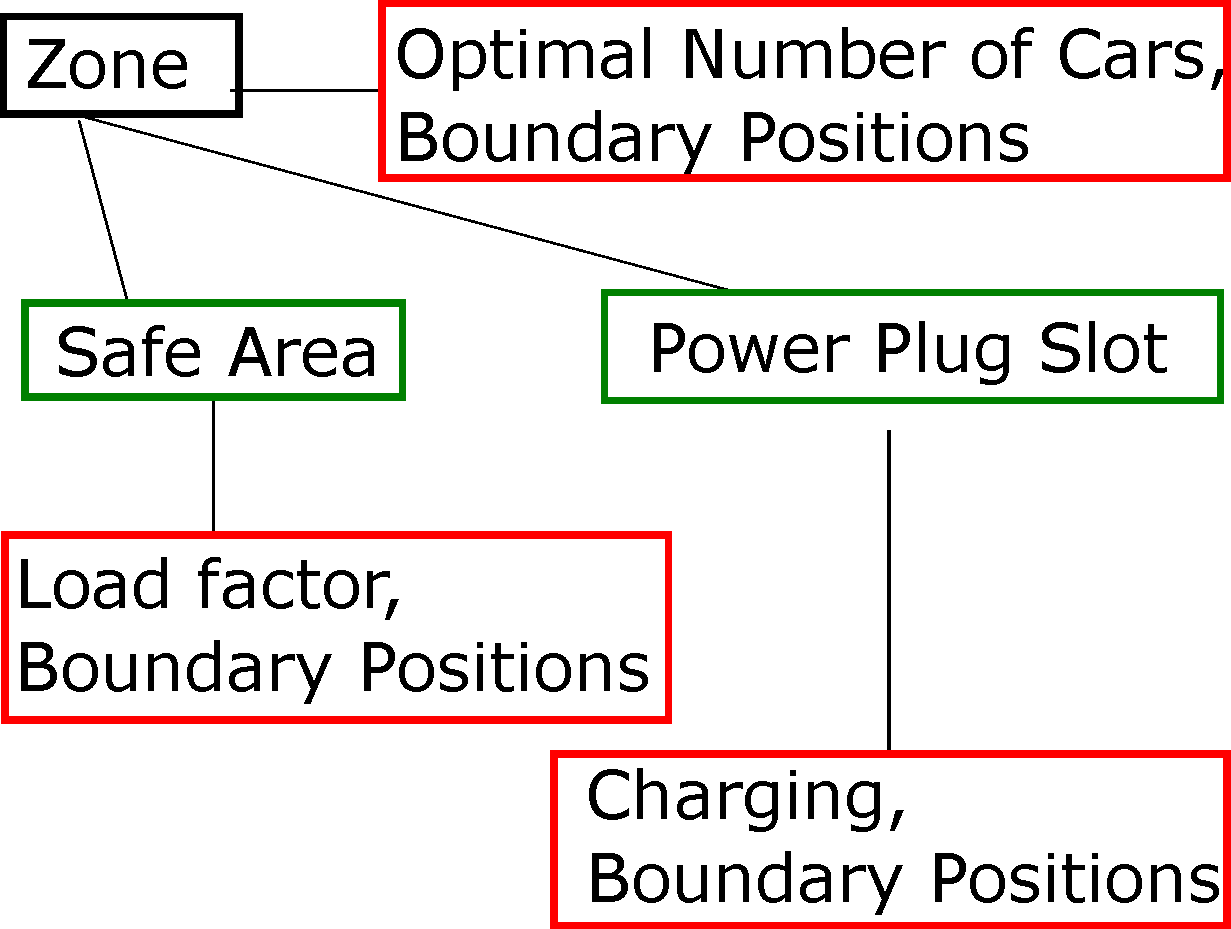
\includegraphics[scale=0.4]{Images/mapStruct.pdf}% "%" necessario
				\caption{Map data Structure}
				\label{fig:mapStruct}
			\end{figure}
	\item  \textbf{BPM \& Relocations:} Computed Discounts, Pending Relocations, Fuel Consumption Weights, Safe areas info 
	\item  \textbf{Fare and Discounts DSL:}Are all the files that contains the DSL scripts and compiled DSL scripts to compute fare and discounts.
	\item  \textbf{API auth Data:} All the informations about external developers are stored adn the data are strutured in a table containing these info App ID, developer info,  Detailed list about Available API.
\end {enumerate}
given all the data structures just explained above and using ILF related FP table we can come up with this function points analysis.

\pagebreak
\begin{fpcounttable}{ILF}
Reservation data\ill\\
Rent data\ilh \\
Payment data\ill\\
Car data\ila \\
User data \ill\\
Staff data\ila \\
Map data\ilh \\
BPM \& Relocations data\ila\\
Fare and Discounts data \ill\\
API auth data\ill\\\hline
\fptotal{95}	
\end{fpcounttable}

\subsubsection{External Interface Files (EIFs)}
\powerenjoy uses EIF in order use external services.
We have identified at least 5 categories of EIF that will be necessary.

\begin {enumerate}
	\item \textbf{Google Map:} Are the files needed to getthe Google Maps API's working, especially for Maps JavaScript API, Google Maps Geocoding API, Google Places API, GoogleMaps Geolocation API, Google Maps Directions API
	\item \textbf{Car Navigation:} these are used to compute path, find safe areas, and all the operations  needed for  the service
	\item \textbf{Car Controller:}  All  the info retrieved from the  car Controller, these are Car status, sensor data, position, number of passengers. The stucture of this data is complex especially for the sensor data and are continuously  send from the cars to the system.
	\item \textbf{Payment:} Are the data of the credit card that the external pyment service needs in order to perform the payment.
	\item \textbf{Document Validation:} Are the documents data that are passed to the external  service in order to make the validation possible.
\end {enumerate}
given all the data structures just explained and using EIF related FP table we can come up with this function points analysis.
\begin{fpcounttable}{EIF}
Google Map\ello x3 \\
Car Navigation\ello \\
Car Controller\elh \\
Payment \ello\\
Document Validation \ello\\\hline
\fptotal{40}	
\end{fpcounttable}

\subsubsection{External Inputs (EIs)}
\powerenjoy service supports many kind of interaction features with different categories of users.
Especially we have found 6 categories of users.
\begin{enumerate}
\item All users:
\begin{itemize}
\item \textbf{Login/Logout} simple operation for each type of user.
\item  \textbf{password retrieval} average complexity operation performed by each type of user, as it involves a number of steps in order to be sure the user is really entitled to retrieve his password. For this reason, it contributes 4 FPs for each type of user.
\end{itemize}
\item \powerenjoyuser:
\begin{itemize}
\item \textbf{Reserve} average complexity operation because it includes the elaboration of the route to the car
\item \textbf{Cancel} low complexity operation because it include a small operation.
\item \textbf{Rent} this operation is divided in sub-operations each one has its contribute to the FP's definition. Each one has a Low complexity apart of Charge operation. It involves the interaction with the power plug slot and it is classified Average.
	\begin{itemize}
		\item Start 
		\item Unlock
		\item Stopover
		\item Park
		\item Charge
	\end{itemize}
\item\textbf{Register} Classified as high complexity operation because it includes a lot of data to be inserted and involves the call to external services for document verification.
\item\textbf{Update info} As the registration it can involve a lot of operations in the backend
\item\textbf{Recover Pin} An average complexity procedure because it involves the response by the system and the generation of the new code.
\end{itemize}
\item External Developers:
\begin{itemize}
\item \textbf{New App} A low complexity operation. 
\end{itemize}
\item Emergency Staff:
\begin{itemize}
\item \textbf{Assign to Field Staff} classified as average because of the interaction with component that it implies.
\item \textbf{Set Car Availability} classified as low because it only changes the car status
\end{itemize}
\item Field Staff:
\begin{itemize}
\item \textbf{Unlock Car} Classified as low because they open the car using their passepartout.
\item \textbf{Start Engine} Classified as low because it implies only the pin insertion
\end{itemize}
\item Management Staff:
\begin{itemize}
\item \textbf{Modify}
	\begin{itemize}
	\item\textit{Discount} defined High because it is a complex object to be  configured
	\item \textit{Fare} defined High because it is a complex object to be  configured
	\item \textit{City Zone} Defined low because it is not so difficult to be configured
	\item \textit{Safe Area} Defined as average because you have to insert set of coordinates
	\item \textit{power plug} Defined as average because you have to insert set of coordinates
	\item \textit{Car}  Defined low because it is not so difficult to be configured 
	\item \textit{term of conditions}  Defined low because it is not so difficult to be configured
	\item \textit{staff account} Defined as average because you have to insert define a lot of informations
	\item \textit{grant/ remove privilege}  defined  High because it is a complex object to be configured
	\end{itemize}
\end{itemize}
\end{enumerate}

\pagebreak
\begin{fpcounttable}{EI}
Login/Logout \eil x12 \\
Password retrieval \eia x6 \\
Reserve \eia \\
Cancel \eil \\
Money Saving Option \eil \\
Rent& - & - \\
-Start \eil\\
-Unlock \eil\\
-Stopover \eil\\
-Park \eil\\
-Charge \eia\\
Register \eih\\
Update info \eih\\
Recover Pin \eia\\
New App \eil\\
Assign to field staff \eia\\
Set Car Availability \eil\\
Unlock car\eil\\
Sart engine\eil\\
Modify &-&-\\
-Discount \eih\\
-Fare \eih\\
-city zone \eil\\
-safe area \eia\\
-power plug\eia\\
-car\eil\\
-term of conditions\eil \\
-staff account\eia\\
-grant/ remove privilege\eih\\\hline 

\fptotal{157}	
\end{fpcounttable}

\subsubsection{External Inquiries (EQs)}
As specied by the FP guidelines, an inquiry is essentially a data retrieval request performed by an user.
\powerenjoy supports interactions of this type:
\begin{itemize} 
	\item \powerenjoyuser must be able to Retrieve near cars
	\item \powerenjoyuser must be able to Retrieve Reserved Car position
	\item emergency \staff must be able to Retrieve Task
	\item field \staff must be able to Retrieve Manteinance/Relocation Requests 
	\item field \staff must be able to Retrieve assigned cars 
	\item emergency\staff and field \staff must be able to Retrieve Car info
	\item \thirdparty developers must be able to Retrieve app privileges
	\item all users must be able to Retrieve map info 
\end{itemize}
The resulting table is the following:
\begin{fpcounttable}{EQ}
Retrive near cars \eih \\
Retrieve Reserved Car position \eil \\
Retrieve Task \eia \\
Retrieve Manteinance/Relocation Requests  \eia x2\\
Retrieve assigned cars \eil\\
Retrieve Car info \eia x2\\
Retrieve app privileges\eih \\
Retrieve map info \eil x6\\ \hline 
\fptotal{56}	
\end{fpcounttable}

\subsubsection{External Outputs (EOs)}
As part of its normal behavior, \powerenjoy service occasionally needs to communicate with the user outside the context of an inquiry. These occasions are:
\begin{itemize}
	\item Notify emergency \staff of the raise of a New Emergency
	\item Notify Field \staff of a New Manteinance request 
	\item Notify field \staff a New Relocation Request
	\item Notify \powerenjoy users of Updated Fare/Terms Of Service/Discounts
	\item Display Rent Info in the car
	\item Notify the \powerenjoyuser sending a Reservation Reminder
	\item Notify Staff for not Payed Rents
\end{itemize}
\pagebreak
\begin{fpcounttable}{EO}
New Emergency\eol\\
New Manteinance request \eol\\
New Relocation Request\eol\\
Update Fare/Terms Of Service/Discounts \eol x3\\
Rent Info in cars \eoa\\
Reservation Reminder\eol\\
Suspension for Rent not Payed\eoh\\\hline 
\fptotal{40}	
\end{fpcounttable}

\subsubsection{Overall estimation}
The following table summarizes the results of our estimation activity:

\begin{fptotaltable}
	Internal Logic Files & 95 \\
	External Logic Files & 40 \\
	External Inputs & 147 \\
	External Inquiries & 56 \\
	External Outputs & 40 \\\hline
	Total & 378\\\hline
\end{fptotaltable}
Given 378 as total FP estimation we calculate the Source Line Of Code using J2EE parameters as follows:
\begin{lstlisting}[stepnumber=0]
	SLOC = 378 * 46 = 17388
\end{lstlisting}
and an upper bound of
\begin{lstlisting}[stepnumber=0]
	SLOC = 378 * 67 = 25326
\end{lstlisting}

\subsection{Cost and effort estimation: COCOMO II}
\subsubsection{Scale Drivers}
In order to evaluate the values of the scale drivers, we refer to the following official COCOMO II table:

\pagebreak
\begin{scaledriverstable}{Scale Factor values, SF$_j$, for COCOMO II Models}
	Scale Factors & Very Low & Low & Nominal & High & Very High & Extra High\\\hline
	\addfactor{PREC}{thoroughly unprecedented}{largely unprecedented}{somewhat unprecedented}{generally familiar}{largely familiar}{thoroughly familiar}
	\addfactorvalues{6.20}{4.96}{3.72}{2.48}{1.24}{0.00}
	\addfactor{FLEX}{rigorous}{occasional relaxation}{some relaxation}{general conformity}{some conformity}{general goals}
	\addfactorvalues{5.07}{4.05}{3.04}{2.03}{1.01}{0.00}
	\addfactor{RESL}{little (20\%)}{some (40\%)}{often (60\%)}{generally (75\%)}{mostly (90\%)}{full (100\%)}
	\addfactorvalues{7.07}{5.65}{4.24}{2.83}{1.41}{0.00}
	\addfactor{TEAM}{very difficult interactions}{some difficult interactions}{basically cooperative interactions}{largely cooperative}{highly cooperative}{seamless interactions}
	\addfactorvalues{5.48}{4.38}{3.29}{2.19}{1.10}{0.00}
	\addfactor{PMAT}{Level 1 Lower}{Level 1 Upper}{Level 2}{Level 3}{Level 4}{Level 5}
	\addfactorvalues{7.80}{6.24}{4.68}{3.12}{1.56}{0.00}
\end{scaledriverstable}
The results of our evaluation is the following:
\begin{factorcounttable}{Scale Driver}
	Precedentedness (PREC) & Nominal & 3.72\\
	Development flexibility (FLEX) & High & 2.03\\
	Risk resolution (RESL) & Low & 5,65\\
	Team cohesion (TEAM) & High & 2,19\\
	Process maturity (PMAT) & Low & 6,24\\\hline
	\fptotal{19,83}
\end{factorcounttable}

\subsubsection{Cost Drivers}
\begin{itemize}
	\item  Required Software Reliability:
	\begin{itemize}
	\item[] Since the system represents the only way to reserve, unlock and use cars it must reliable 24/7 so we set this parameter as High.
	\pagebreak
	\begin{costdriverstable}{RELY Cost Drivers}
		\costdescriptors{RELY Descriptors}{slightly inconvenience}{easily recoverable losses}{moderate recoverable losses}{high financial loss}{risk to human life}{}\hline
		\ratinglevel{Very low}{Low}{Nominal}{High}{Very High}{Extra High}
		\effortmultipliers{0.82}{0.92}{1.00}{1.10}{1.26}{n/a}
	\end{costdriverstable}
	\end{itemize}
\end{itemize}

\begin{itemize}
	\item Database size:
	\begin{itemize}
	\item[] This measure attempts to capture the affect large data requirements have on product development. The reason the size of the database is important to consider it because of the effort required to generate the test data that will be used to exercise
the program. \par The value will be set to \textit{nominal}.
	\begin{costdriverstable}{DATA Cost Drivers}
		\costdescriptors{DATA Descriptors}{}{$\frac{D}{P}$ $<$ 10}{10 $\le$ $\frac{D}{P}$ $\le$ 100}{100 $\le$ $\frac{D}{P}$ $\le$ 1000}{$\frac{D}{P}$ $>$ 1000}{}\hline
		\ratinglevel{Very low}{Low}{Nominal}{High}{Very High}{Extra High}
		\effortmultipliers{n/a}{0.90}{1.00}{1.14}{1.28}{n/a}
	\end{costdriverstable}
	\end{itemize}
\end{itemize}
In accordance with the new COCOMO II CPLEX rating scale, this value will be high.
\begin{itemize}
	\item Product complexity: 
	\begin{itemize}
	\item[] Set to very high according to the COCOMO II rating scale.
	\begin{costdriverstable}{CPLX Cost Driver}
		\ratinglevel{Very low}{Low}{Nominal}{High}{Very High}{Extra High}
		\effortmultipliers{0.73}{0.87}{1.00}{1.17}{1.34}{1.74}	
	\end{costdriverstable}
	\end{itemize}
\end{itemize}

\begin{itemize}
	\item Required reusability: 
	\begin{itemize}
	\item[] This cost driver accounts for the additional effort needed to construct components intended for reuse on the current or future projects. This effort is consumed with creating more generic design of software, more elaborate documentation, and more extensive testing to ensure components are ready for use in other applications.
We have chosen a \textit{nominal} value because the architecture is quite dependent to the goals required.
	\begin{costdriverstable}{RUSE Cost Driver}
		\costdescriptors{RUSE Descriptors}{}{None}{Across project}{Across program}{Across product line}{Across multiple product lines}\hline
		\ratinglevel{Very low}{Low}{Nominal}{High}{Very High}{Extra High}
		\effortmultipliers{n/a}{0.95}{1.00}{1.07}{1.15}{1.24}		
	\end{costdriverstable}
	\end{itemize}
\end{itemize}

\begin{itemize}
	\item Documentation match to life-cycle needs: 
	\begin{itemize}
	\item[] In accordance with the new COCOMO II DOCU rating scale, this value will be \textit{high}.
	\begin{costdriverstable}{DOCU Cost Driver}
		\costdescriptors{DOCU Descriptors}{Many life-cycle needs uncovered}{Some life-cycle needs uncovered}{Right-sized to life-cycle needs}{Excessive for life-cycle needs}{Very excessive for life-cycle needs}{}\hline
		\ratinglevel{Very low}{Low}{Nominal}{High}{Very High}{Extra High}
		\effortmultipliers{0.81}{0.91}{1.00}{1.11}{1.23}{n/a}		
	\end{costdriverstable}
	\end{itemize}
\end{itemize}

\begin{itemize}
	\item Execution time constraint: 
	\begin{itemize}
	\item[] This parameter describes the expected amount of CPU usage with respect to the computational capabilities of the hardware. In accordance with the new COCOMO II TIME rating scale, this value will be \textit{high}.
	\begin{costdriverstable}{TIME Cost Driver}
		\costdescriptors{TIME Descriptors}{}{}{$\le$ 50\% use of available execution time}{70\% use of available execution time}{85\% use of available execution time} {95\% use of available execution time}\hline
		\ratinglevel{Very low}{Low}{Nominal}{High}{Very High}{Extra High}
		\effortmultipliers{n/a}{n/a}{1.00}{1.11}{1.29}{1.63}	
	\end{costdriverstable}
	\end{itemize}
\end{itemize}

\begin{itemize}
	\item Storage constraint: 
	\begin{itemize}
	\item[] This parameter describes the expected amount of storage usage with respect to the availability of the hardware.In accordance with the new COCOMO II STOR rating scale, this value will be high. this value is set to nominal.
	\begin{costdriverstable}{STOR Cost Driver}
		\costdescriptors{STOR Descriptors}{}{}{$\le$  50\% use of available storage}{70\% use of available storage}{85\% use of available storage} {95\% use of available storage}\hline
		\ratinglevel{Very low}{Low}{Nominal}{High}{Very High}{Extra High}
		\effortmultipliers{n/a}{n/a}{1.00}{1.05}{1.17}{1.46}	
	\end{costdriverstable}
	\end{itemize}
\end{itemize}

\begin{itemize}
	\item Platform Volatility: 
	\begin{itemize}
	\item[] For what concerns the core system, we don't expect our fundamental platforms to change very often. However, the client applications may require at least a major release once every six months to be aligned with the development cycle of the main mobile operating systems. For this reason, this parameter is set to nominal.
	\begin{costdriverstable}{PVOL Cost Driver}
		\costdescriptors{PVOL Descriptors}{}{Major change every 12 mo., minor change every 1 mo.}{Major: 6mo; minor: 2wk.}{Major: 2mo, minor: 1wk}	{Major: 2wk; minor: 2 days}{}\hline
		\ratinglevel{Very low}{Low}{Nominal}{High}{Very High}{Extra High}
		\effortmultipliers{n/a}{0.87}{1.00}{1.15}{1.30}{n/a}
	\end{costdriverstable}
	\end{itemize}
\end{itemize}

\begin{itemize}
	\item Analyst Capability: 
	\begin{itemize}
	\item[] In accordance with the new COCOMO II ACAP rating scale, this value will be \textit{low}.
	\begin{costdriverstable}{ACAP Cost Driver}
		\costdescriptors{ACAP Descriptors}{15th percentile}{35th percentile}{55th percentile}{75th percentile}{90th percentile}{}\hline
		\ratinglevel{Very low}{Low}{Nominal}{High}{Very High}{Extra High}
		\effortmultipliers{1.42}{1.19}{1.00}{0.85}{0.71}{n/a}	
	\end{costdriverstable}
	\end{itemize}
\end{itemize}

\begin{itemize}
	\item Programmer Capability: 
	\begin{itemize}
	\item[]  In accordance with the new COCOMO II PCAP rating scale, this value will be \textit{low}.
	\begin{costdriverstable}{PCAP Cost Driver}
		\costdescriptors{PCAP Descriptors}{15th percentile}{35th percentile}{55th percentile}{75th percentile}{90th percentile}{}\hline
		\ratinglevel{Very low}{Low}{Nominal}{High}{Very High}{Extra High}
		\effortmultipliers{1.34}{1.15}{1.00}{0.88}{0.76}{n/a}	
	\end{costdriverstable}
	\end{itemize}
\end{itemize}

\begin{itemize}
	\item Application Experience: 
	\begin{itemize}
	\item[]  In accordance with the new COCOMO II APEX rating scale, we rate this parameter as \textit{low}.
	\begin{costdriverstable}{APEX Cost Driver}
		\costdescriptors{APEX Descriptors}{$\le$ 2 months}{6 months}{1 year}{3 years}{6 years}{}\hline
		\ratinglevel{Very low}{Low}{Nominal}{High}{Very High}{Extra High}
		\effortmultipliers{1.22}{1.10}{1.00}{0.88}{0.81}{n/a}
	\end{costdriverstable}
	\end{itemize}
\end{itemize}

\begin{itemize}
	\item Platform Experience: 
	\begin{itemize}
	\item[] We don't have any experience with the Java EE platform. For this reason, we're going to set this parameter to \textit{low}.
	\begin{costdriverstable}{PLEX Cost Driver}
		\costdescriptors{PLEX Descriptors}{$\le$ 2 months}{6 months}{1 year}{3 years}{6 years}{}\hline
		\ratinglevel{Very low}{Low}{Nominal}{High}{Very High}{Extra High}
		\effortmultipliers{1.19}{1.09}{1.00}{0.91}{0.85}{n/a}
	\end{costdriverstable}
	\end{itemize}
\end{itemize}

\begin{itemize}
	\item Language and Tool Experience: 
	\begin{itemize}
	\item[]  In accordance with the new COCOMO II LTEX rating scale, this value will be \textit{high}.
	\begin{costdriverstable}{LTEX Cost Driver}
		\costdescriptors{LTEX Descriptors}{$\le$ 2 months}{6 months}{1 year}{3 years}{6 years}{}\hline
		\ratinglevel{Very low}{Low}{Nominal}{High}{Very High}{Extra High}
		\effortmultipliers{1.20}{1.09}{1.00}{0.91}{0.84}{n/a}
	\end{costdriverstable}
	\end{itemize}
\end{itemize}

\pagebreak
\begin{itemize}
	\item Personnel continuity: 
	\begin{itemize}
	\item[]  In accordance with the new COCOMO II PCON rating scale, this value will be \textit{high}. 
	\begin{costdriverstable}{PCON Cost Driver}
		\costdescriptors{PCON Descriptors}{48\% / year}{24\% / year}{12\% / year}{6\% / year}{3\% / year}{}\hline	
		\ratinglevel{Very low}{Low}{Nominal}{High}{Very High}{Extra High}
		\effortmultipliers{1.29}{1.12}{1.00}{0.90}{0.81}{n/a}
	\end{costdriverstable}
	\end{itemize}
\end{itemize}

\begin{itemize}
	\item Usage of Software Tools: 
	\begin{itemize}
	\item[] Our application environment is complete and well integrated, so we'll set this parameter as \textit{high}. 
	\begin{costdriverstable}{TOOL Cost Driver}
		\costdescriptors{TOOL Descriptors}{edit, code, debug}{simple, frontend, backend CASE, little integration}{basic life-cycle tools, moderately integrated}{strong, mature life-cycle tools, moderately integrated}{strong, mature, proactive life-cycle tools, well integrated with processes, methods, reuse}{}\hline
		\ratinglevel{Very low}{Low}{Nominal}{High}{Very High}{Extra High}
		\effortmultipliers{1.17}{1.09}{1.00}{0.90}{0.78}{n/a}	
	\end{costdriverstable}
	\end{itemize}
\end{itemize}

\begin{itemize}
	\item Multisite development: 
	\begin{itemize}
	\item[]  In accordance with the new COCOMO II SITE rating scale, this value will be \textit{extra high}.
	\pagebreak
	\begin{costdriverstable}{SITE Cost Driver}
		\costdescriptors{SITE Collocation Descriptors}{Intern-ational}{Multi-city and multi-company}{Multi-city or multi-company}{Same city or metro area}{Same building or complex}{Fully collocated}
		\costdescriptors{SITE Communications Descriptors}{Some phone, mail}{Individual phone, fax}{Narrow band email}{Wideband electronic communication}{Wideband elect. comm., occasional video conf.}{Interactive multimedia}\hline
		\ratinglevel{Very low}{Low}{Nominal}{High}{Very High}{Extra High}
		\effortmultipliers{1.22}{1.09}{1.00}{0.93}{0.86}{0.80}		
	\end{costdriverstable}
	
	\end{itemize}
\end{itemize}

\begin{itemize}
	\item Required development schedule: 
	\begin{itemize}
	\item[] In accordance with the new COCOMO II SCED rating scale, this value will be \textit{nominal}.
	\begin{costdriverstable}{SCED Cost Driver}
		\costdescriptors{SCED Descriptors}{75\% of nominal}{85\% of nominal}{100\% of nominal}{130\% of nominal}{160\% of nominal}{}\hline
		\ratinglevel{Very low}{Low}{Nominal}{High}{Very High}{Extra High}
		\effortmultipliers{1.43}{1.14}{1.00}{1.00}{1.00}{n/a}	
	\end{costdriverstable}
	\end{itemize}
\end{itemize}

\pagebreak
Overall, our results are expressed by the following table:
\begin{factorcounttable}{Cost Driver}
	Required Software Reliability (RELY) & High & 1.10\\
	Database size (DATA) & Nominal & 1\\
	Product complexity (CPLX) & High & 1,17\\
	Required Reusability (RUSE) & Nominal & 1.00\\
	Documentation match to life-cycle needs (DOCU) & High & 1,11\\
	Execution Time Constraint (TIME) & High & 1,11 \\
	Main storage constraint (STOR) & Nominal & 1.00 \\
	Platform volatility (PVOL) & High & 1.15 \\
	Analyst capability (ACAP) & Low & 1,19 \\
	Programmer capability (PCAP) & Low & 1,15 \\
	Application Experience (APEX) & Low & 1.10 \\
	Platform Experience (PLEX) & Low & 1.09 \\
	Language and Tool Experience (LTEX) & Highl & 0.91 \\
	Personnel continuity (PCON) & Very high & 0.81 \\
	Usage of Software Tools (TOOL) & High & 0.90 \\
	Multisite development (SITE) & Extr high & 0.80\\
	Required development schedule (SCED) & Nominal & 1.00 \\\hline
	\fptotal{1.58798}
\end{factorcounttable}

\subsubsection{Effort equation}
This final equation gives us the effort estimation measured in Person-Months (PM):
\begin{lstlisting}[mathescape, numbers=none, frame=single]
	Effort = A * EAF * KSLOC$^E$
\end{lstlisting}
where:
\begin{lstlisting}[mathescape, numbers=none, frame=single]
	A = 2.94 (for COCOMO II) 
	EAF = product of all cost drivers (1.58798)
	E = exponent derived from the scale drivers. It is computed as:
		B + 0.01 * $\sum_{i} SF[i]$ = B + 0.01 * 19,83 = 0.91 + 0.1983 = 1.1083
		in which B is equal to: 0.91 for COCOMO II.
\end{lstlisting}

With this parameters we can compute the effort value, which has a lower bound of:
\begin{lstlisting}[mathescape, numbers=none, frame=single]
	Effort = A * EAF * KSLOC$^E$ = 2.94 * 1.58798 * 17.338$^{1.1083}$ = 110,249 PM $\approx$ 110 PM
\end{lstlisting}
and an upper bound of:
\begin{lstlisting}[mathescape, numbers=none, frame=single]
	Effort = A * EAF * KSLOC$^E$ = 2.94 * 1.58798 * 25.326$^{1.1083}$ = 167,79 PM $\approx$ 168 PM
\end{lstlisting}

\subsubsection{Schedule estimation}
In order to estimate the real project timespan, we should divide the effort by the members' number (divide by 3 in our case).
\begin{lstlisting}[mathescape, numbers=none]
	Effort = 110,249 PM 
	Duration  = 110,249 PM / 3 = 36,74 months 
	
	Effort = 167,79 PM
	Duration  = 167,79 PM / 3 = 55,93 months 
\end{lstlisting}
We think this excessively wide timespan (4 years and 6 months) is incompatible with the business viability of the project, in fact all the assumptions made in the early analysis could became invalid because of new competitors or changes in laws and regulations.
Thus we need to hire qualified staff to reduce project's timespan to a reasonable amount (time to market).
\par Cocomo II provides us with the right set of formulas to estimate a feasible and reasonable time to market for our project, non-regarding on the number of people working on the project. We can divide the effort by this computed time to market to decide how many people to hire (approximately) to finish in that time.

Cocomo II's results are:
\begin{lstlisting}[mathescape, numbers=none]
	Duration = 3.67 * Effort$^F$
\end{lstlisting}
As a lower bound, we consider
\begin{lstlisting}[mathescape, numbers=none]
	F = 0.28 + 0.2 * (E - B) = 0,31966
	Effort = 110,249 PM 
	Duration = 3.67 * (110,249)$^{0,31966}$ = 16,5 months
\end{lstlisting}
while as an upper bound, we consider
\begin{lstlisting}[mathescape, numbers=none]
	F = 0.28 + 0.2 * (E - B) = 0,31966
	Effort = 167,789 PM 
	Duration = 3.67 * (167,789)$^{0,31966}$ = 18,9 months
\end{lstlisting}
\begin{figure}[H]
			\centering
			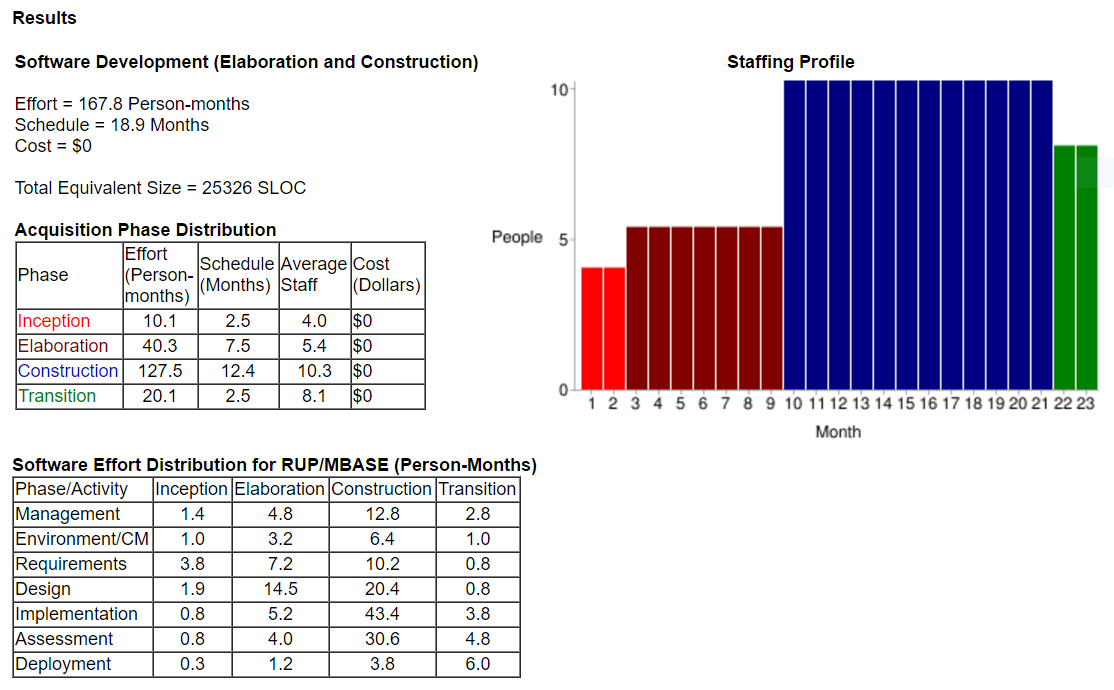
\includegraphics[scale=0.55]{./Images/COCOMOutput18.png} 
		\end{figure}


From this result we can estimate in normal estimation and upper bound cases:
\begin{lstlisting}[mathescape, numbers=none]
 People = Effort / Duration 
	= 110,249 PM / 16.5 months 
	= 6.68 (approx 7 people)
\end{lstlisting}
\begin{lstlisting}[mathescape, numbers=none]
 People = Effort / Duration 
	= 167,789 PM / 18,9 months 
	= 8.87 (approx 9 people)
\end{lstlisting}
Therefore we could hire additional 5 people to be able to go to market in approximately 16.5 months (with an uncertainty of 2 months).
In case of delay, we could mitigate by balancing the amount of features in each one of the planned 3 releases.

\section{Schedule}
	In this section we are going to present a probable project schedule. Obviously this is a prototype and will be refined during the development. \\
	In order to mantain readability and to allow a better understanding, the project schedule will be first presented in a global way and then each part will be expanded.
		\begin{landscape}
	\subsection{Global}
		\begin{figure}[H]
			\centering
			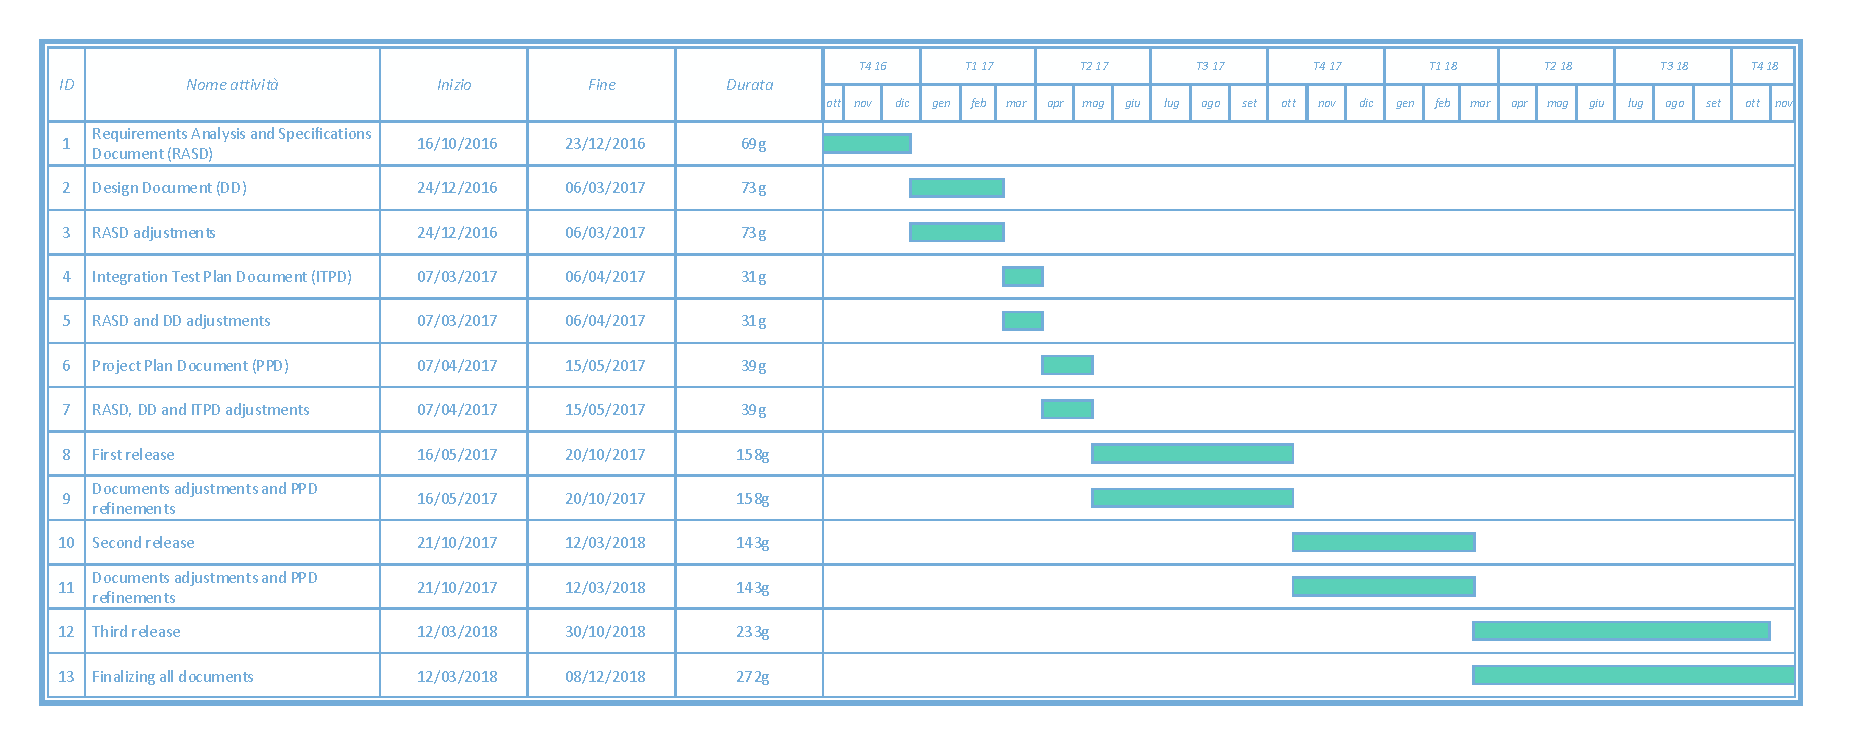
\includegraphics[scale=0.675]{Images/0-Global18.pdf} 
		\end{figure}
		\end{landscape}
	\subsection{RASD}
		\begin{figure}[H]
			\centering
			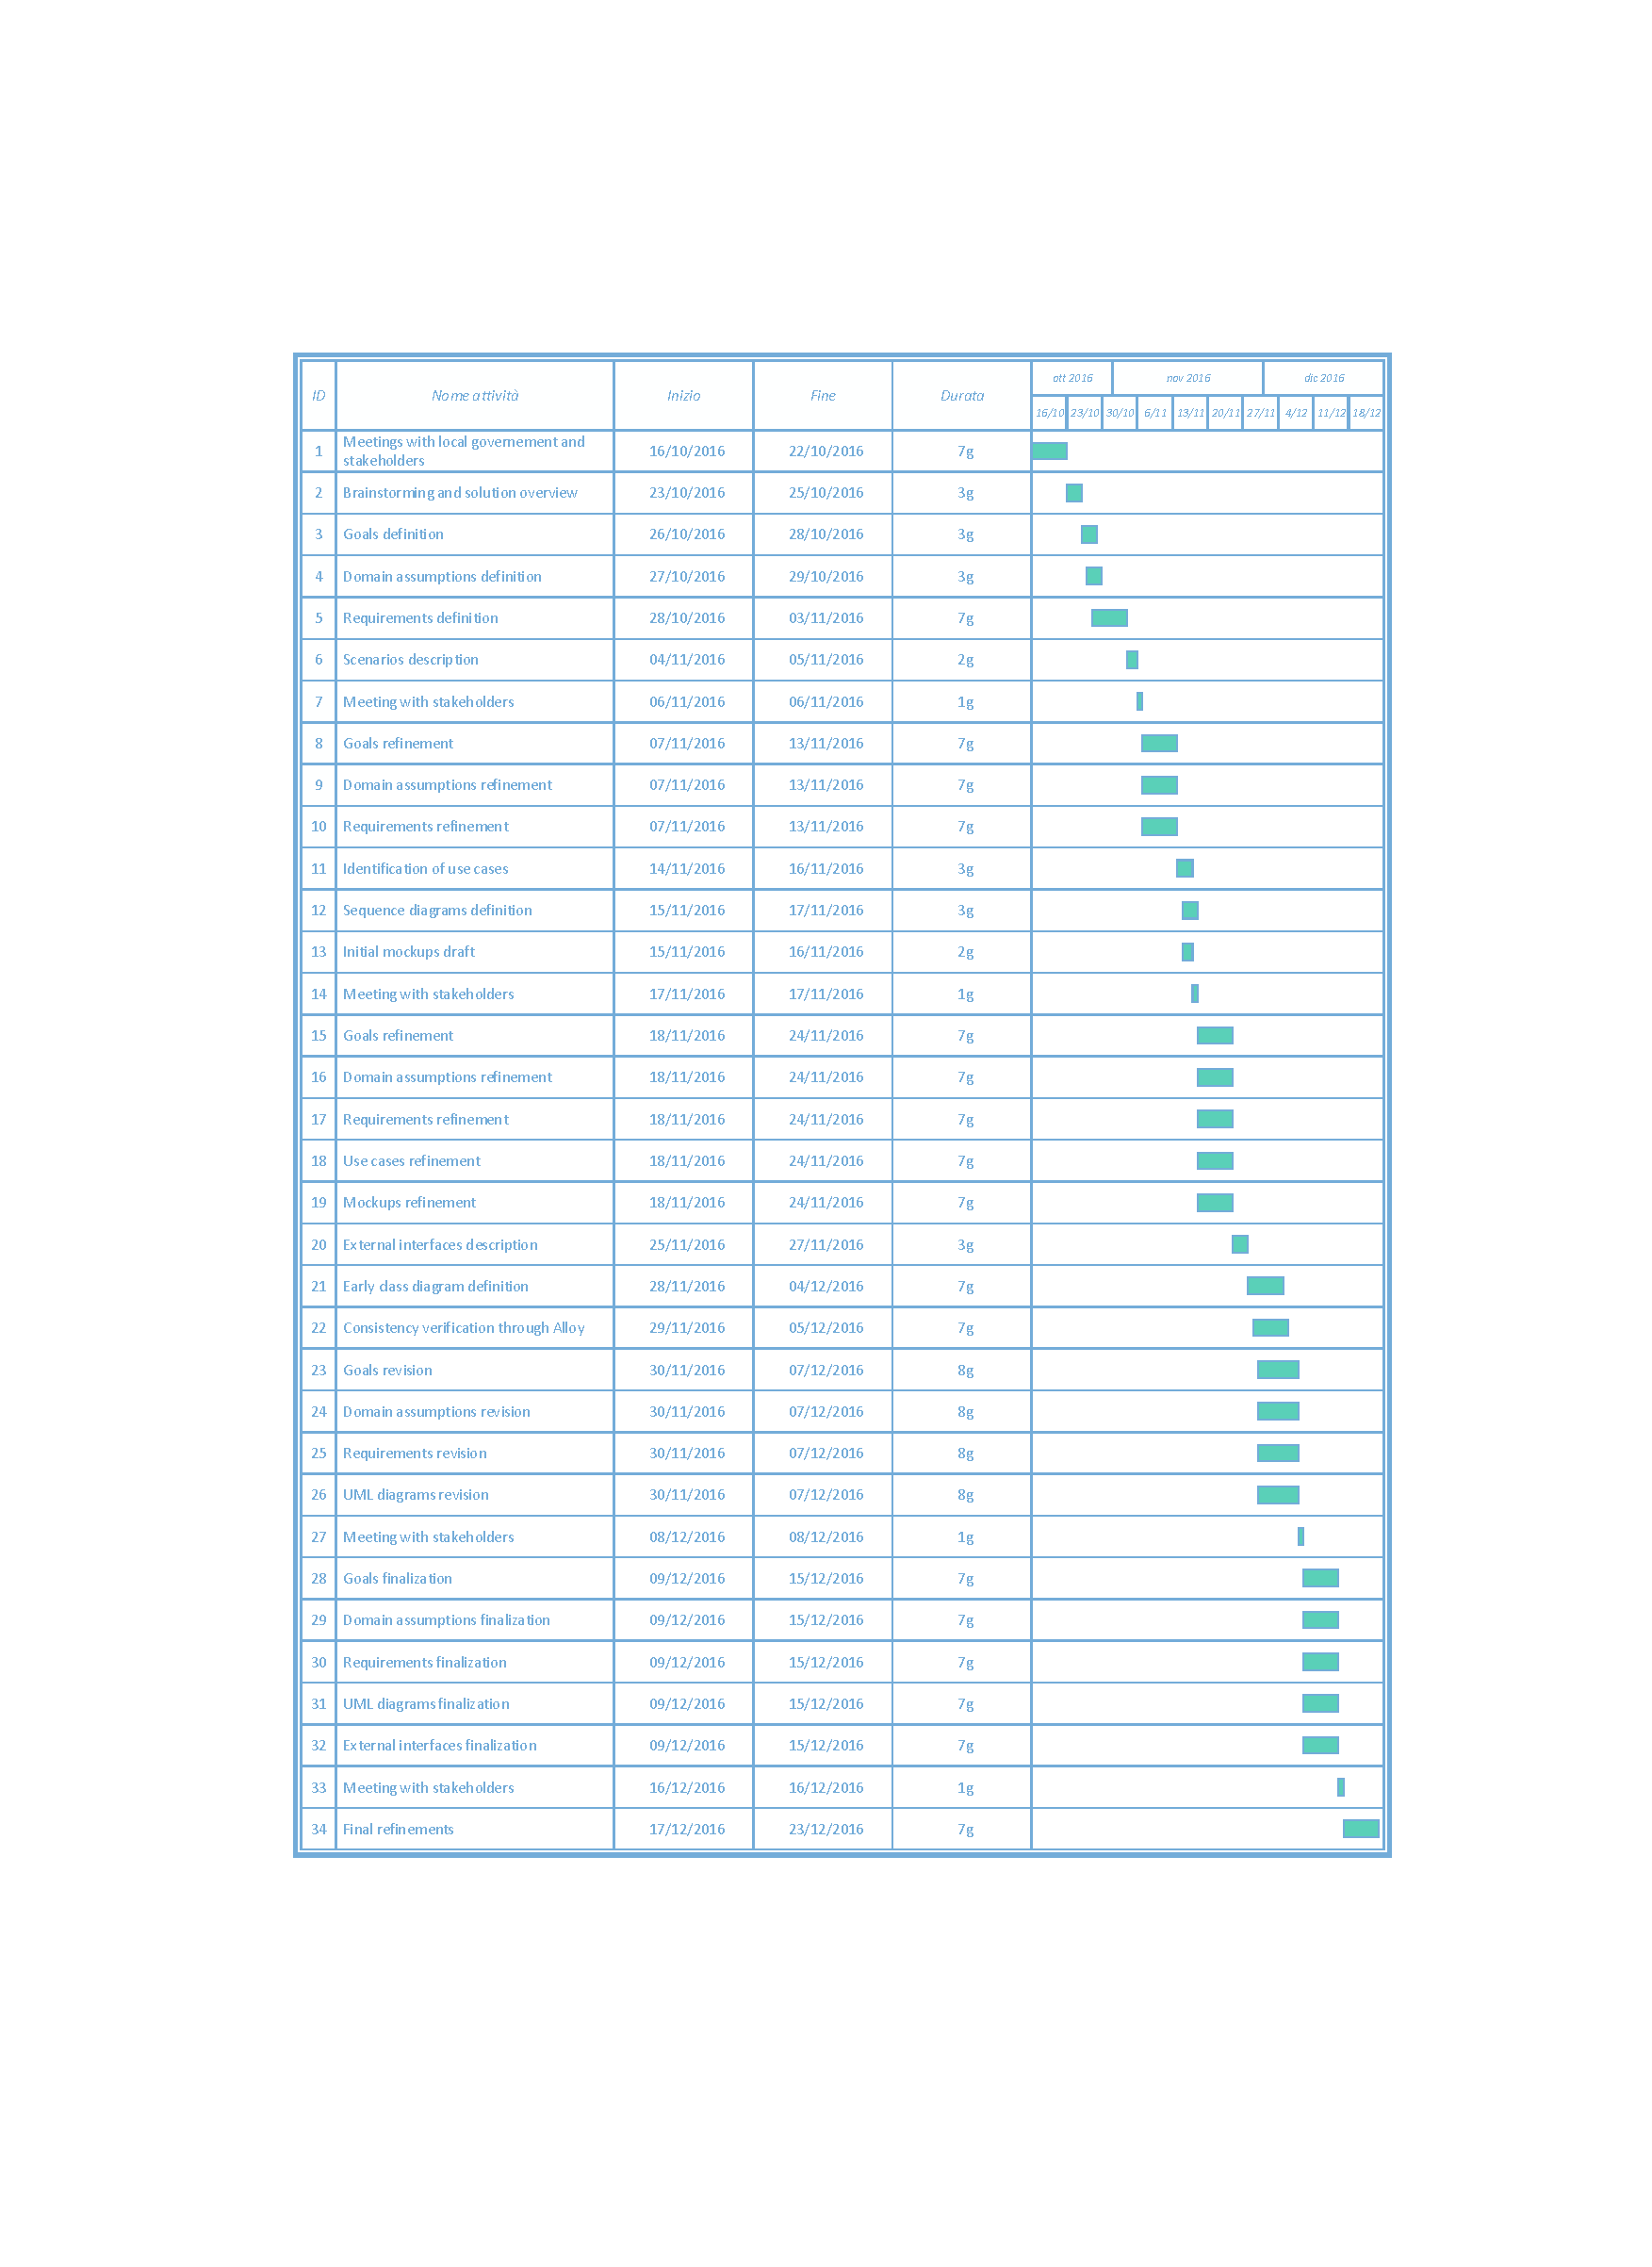
\includegraphics[scale=0.55]{./Images/1-RasdGantt.pdf} 
		\end{figure}
	\subsection{DD}
		\begin{figure}[H]
			\centering
			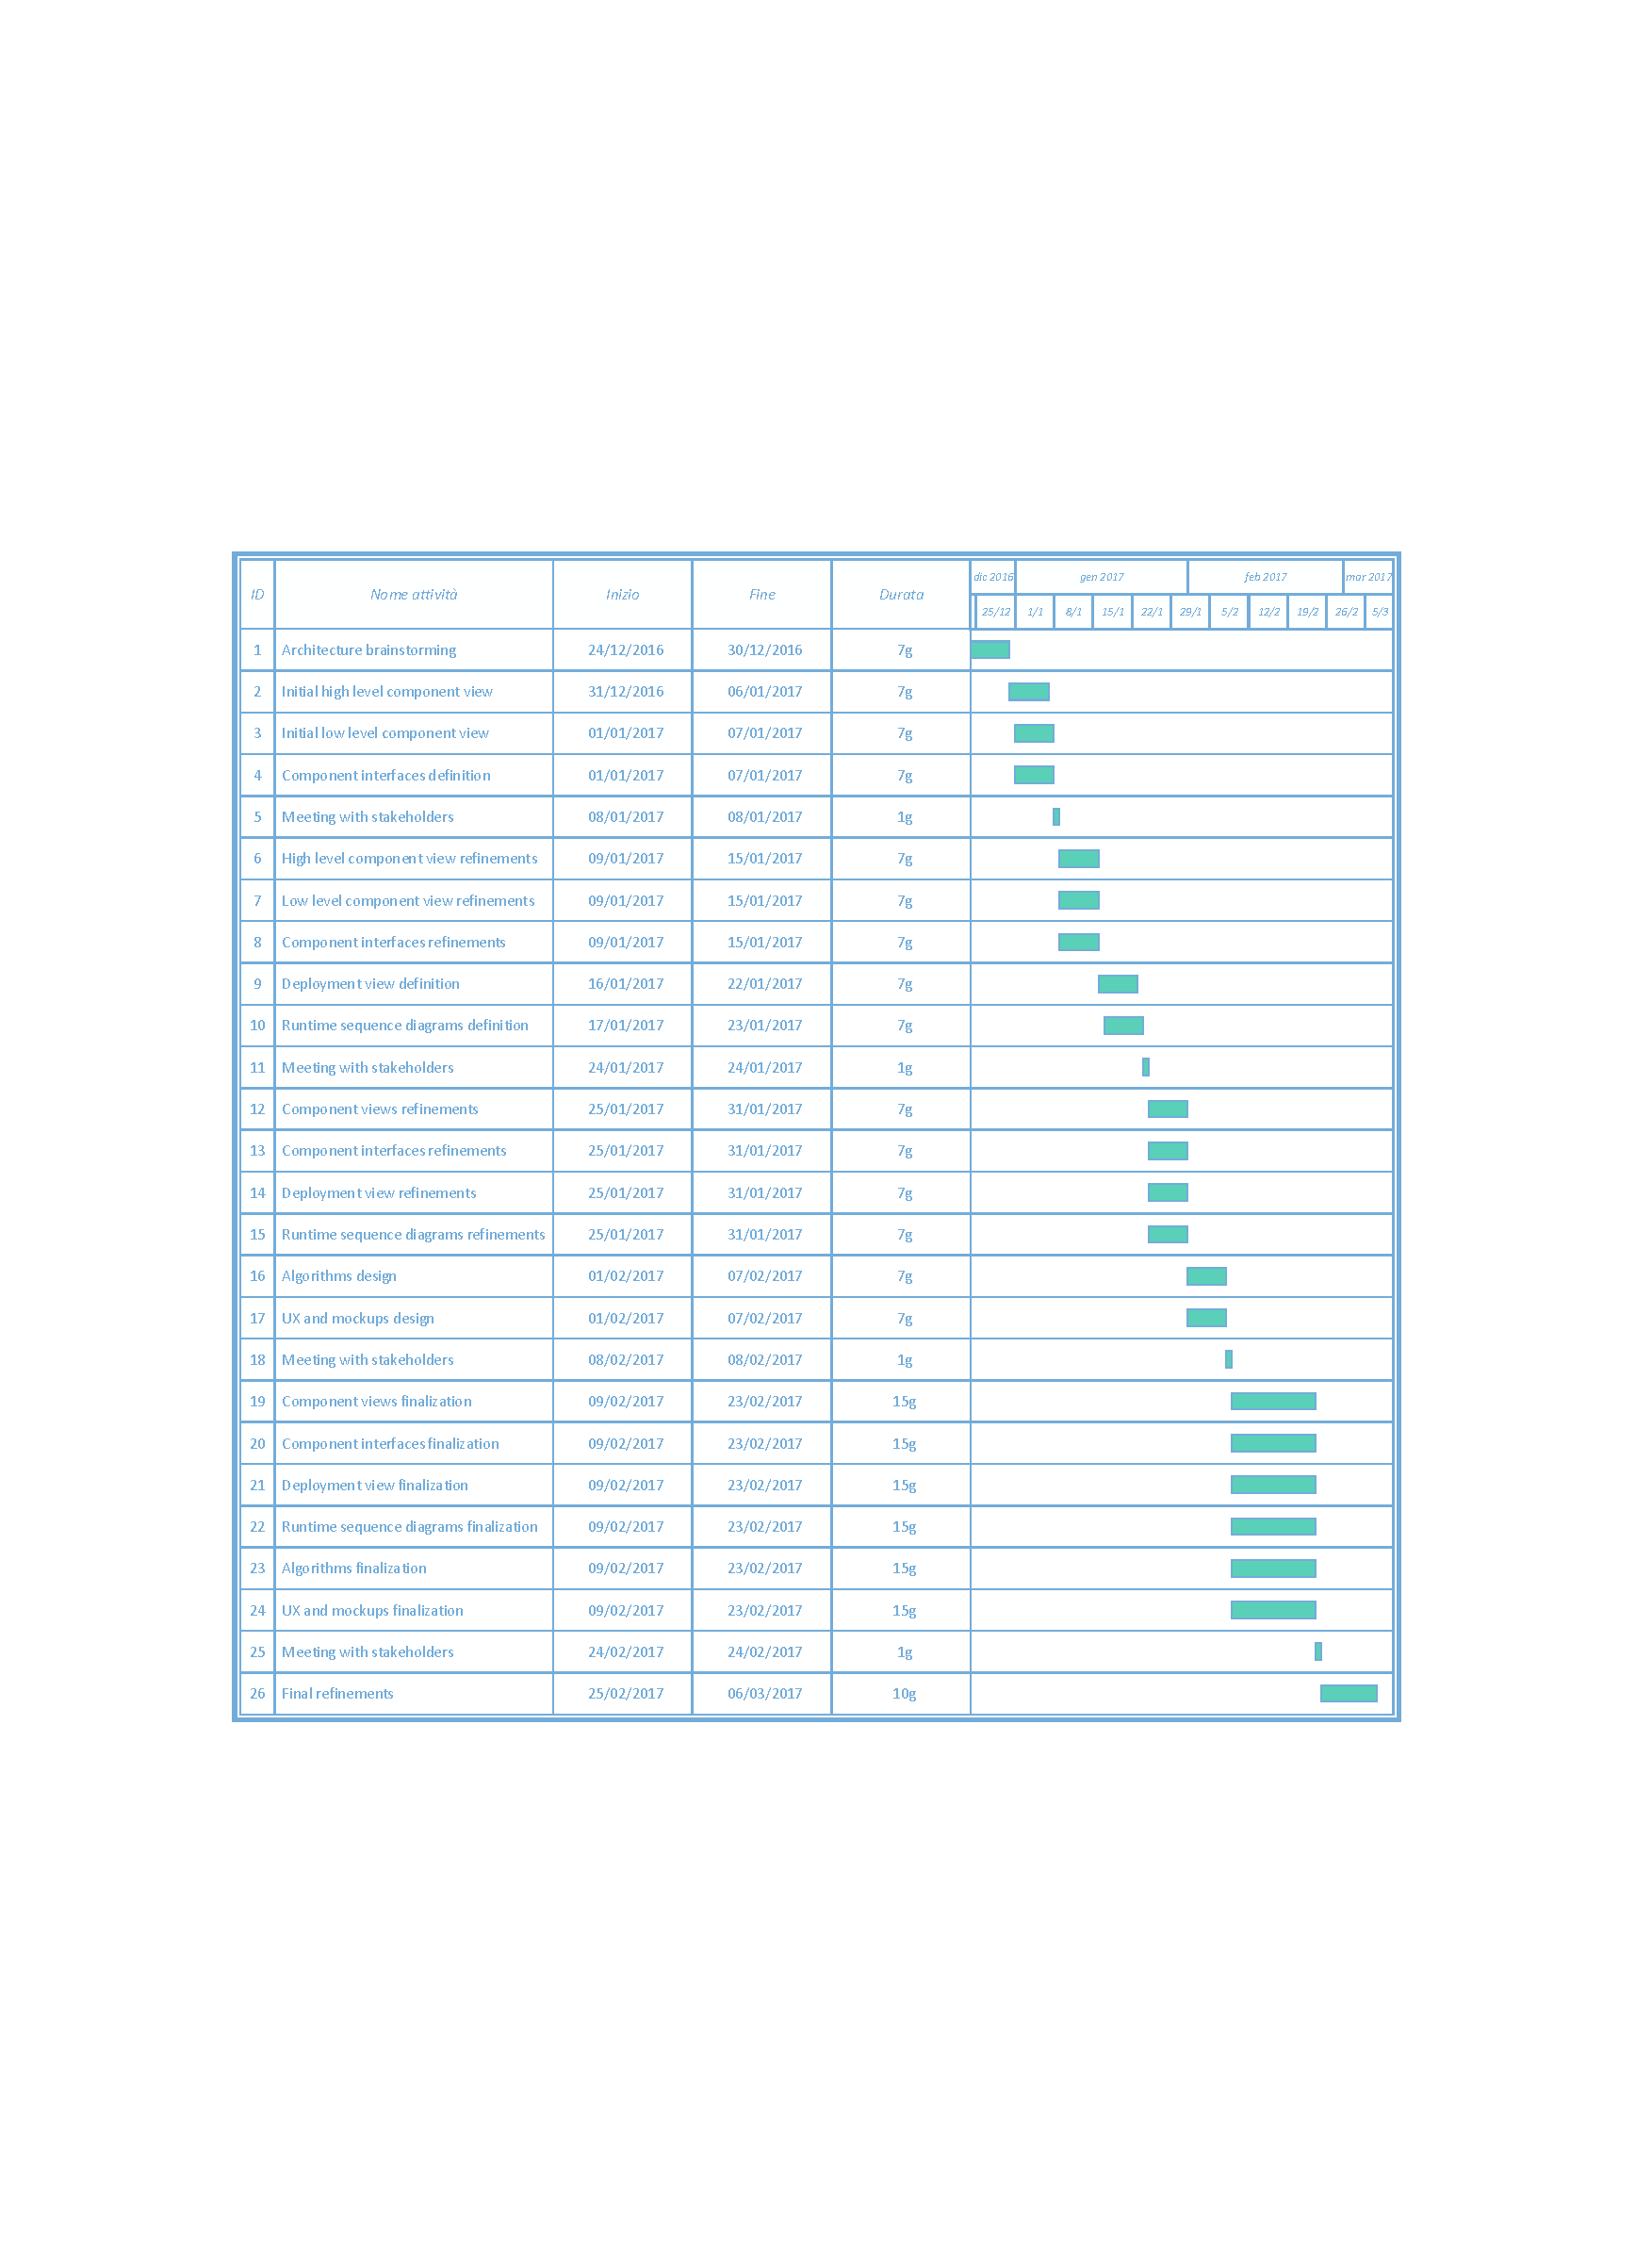
\includegraphics[scale=0.5]{./Images/2-DDGantt.pdf} 
		\end{figure}
		\begin{landscape}
	\subsection{IT}
		\begin{figure}[H]
			\centering
			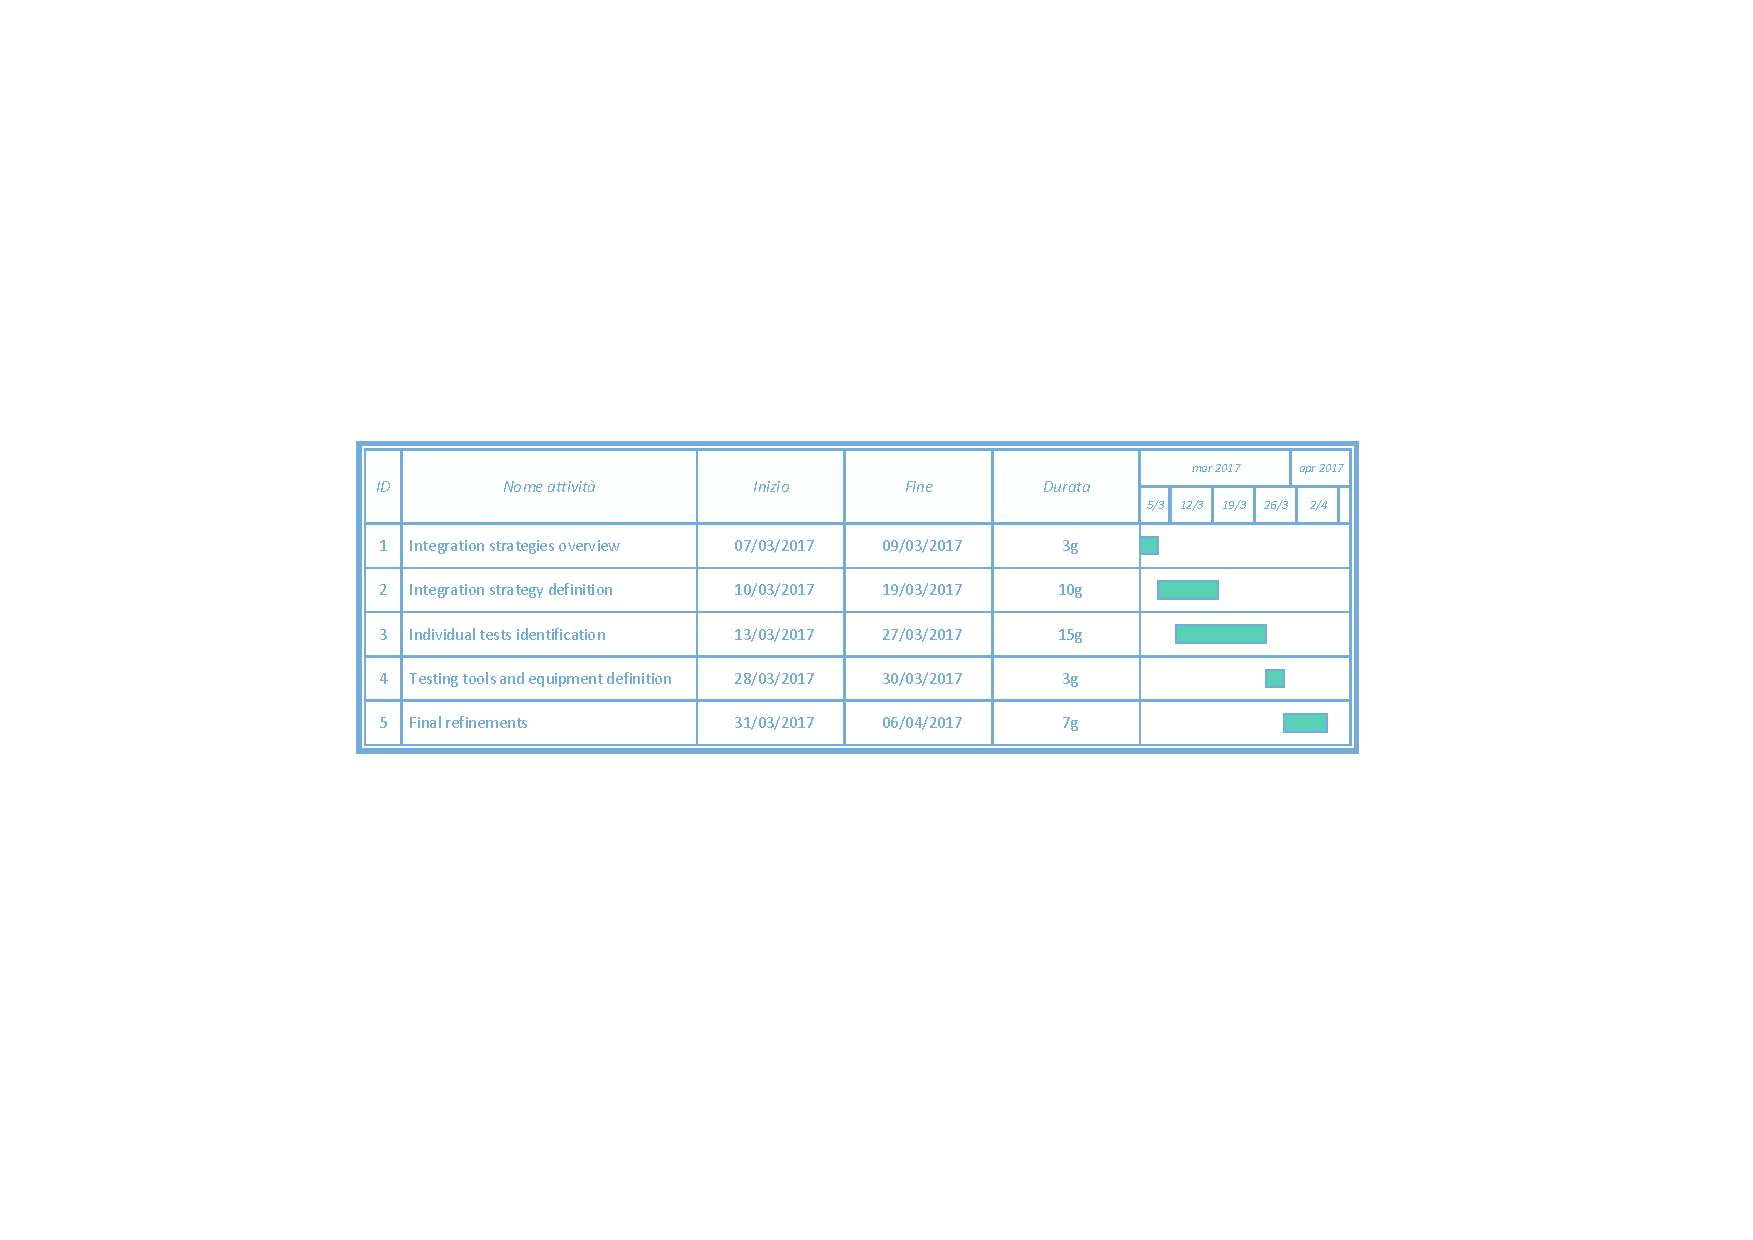
\includegraphics[scale=0.75]{./Images/3-ITGantt.pdf} 
		\end{figure}
		\end{landscape}
		\begin{landscape}
	\subsection{PP}
		\begin{figure}[H]
			\centering
			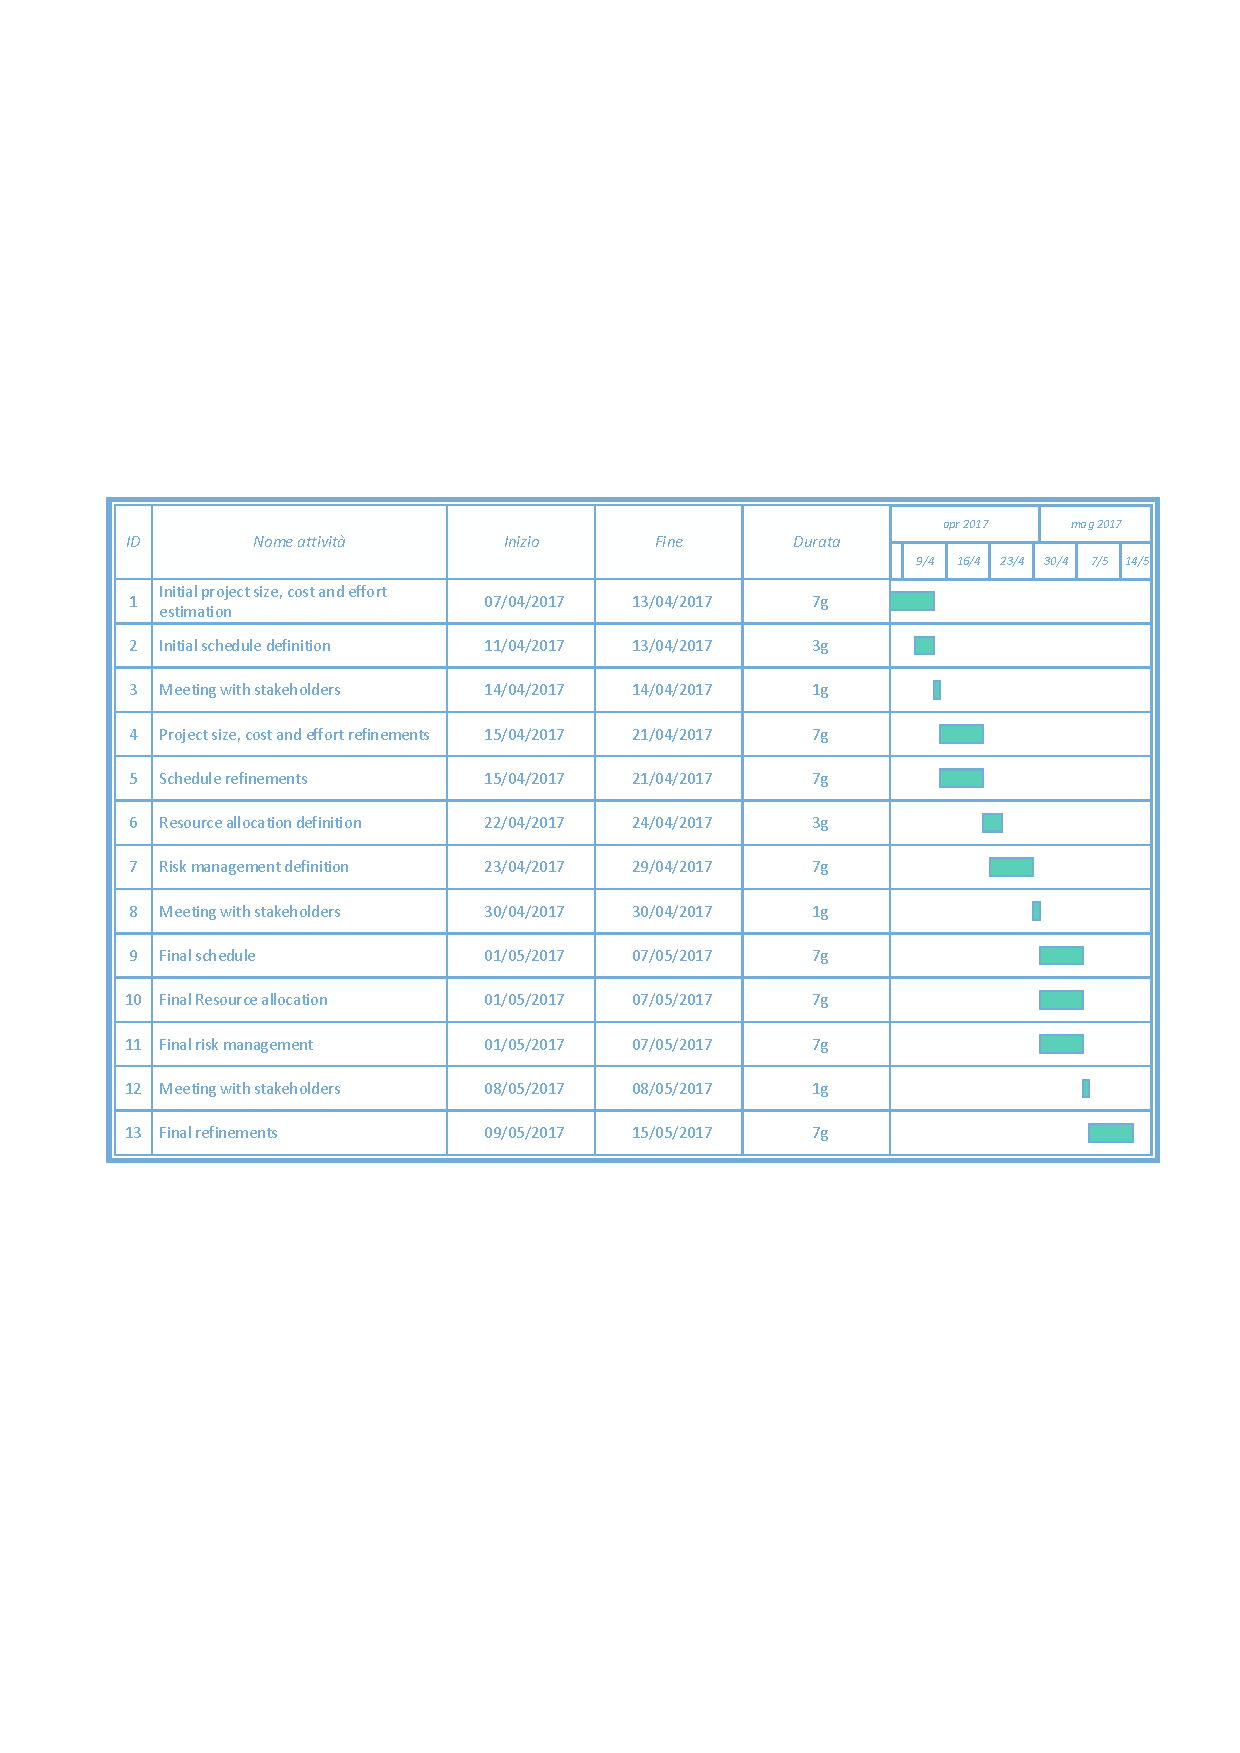
\includegraphics[scale=0.6]{./Images/4-PPGantt.pdf} 
		\end{figure}
		\end{landscape}
		\begin{landscape}
	\subsection{First release}
		\begin{figure}[H]
			\centering
			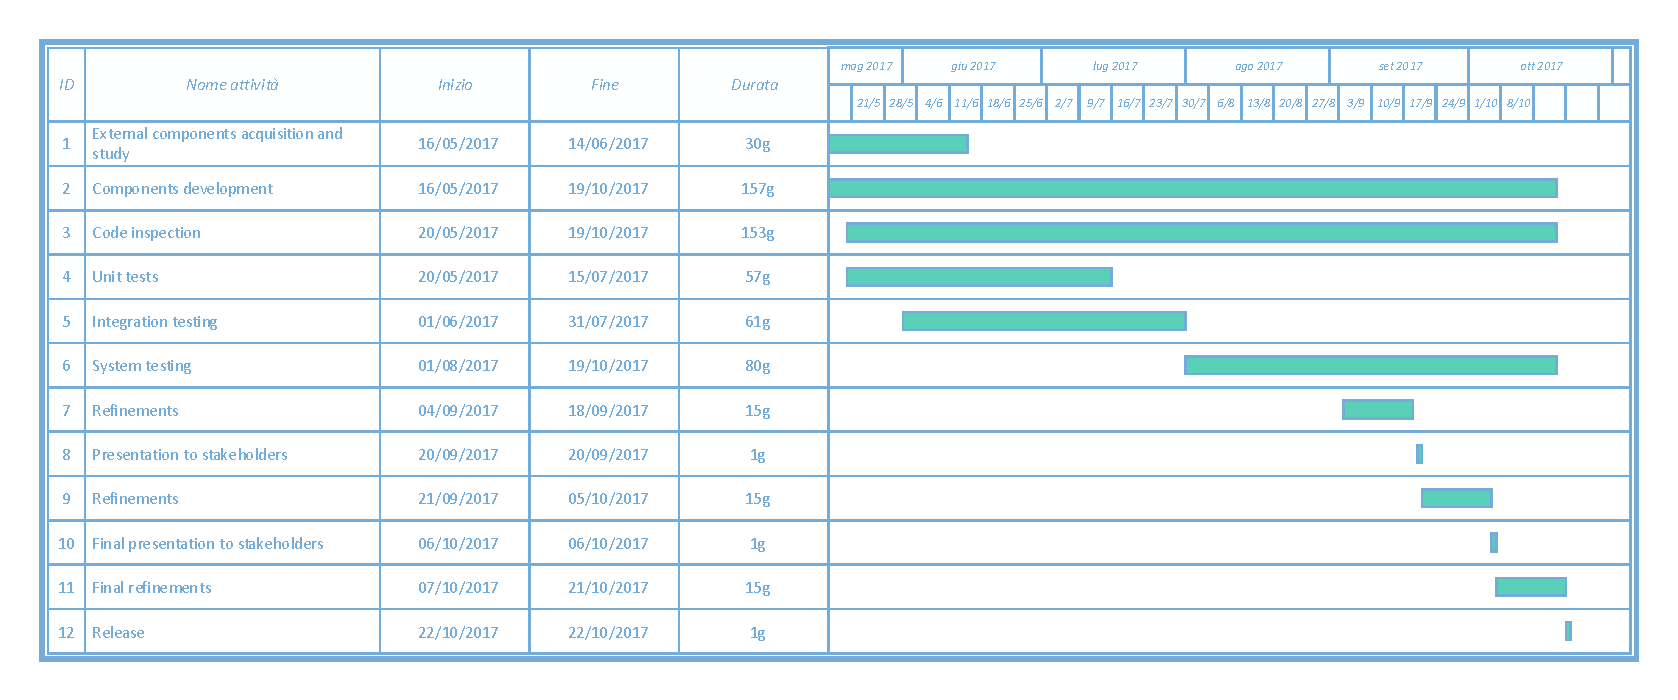
\includegraphics[scale=0.725]{./Images/5-FirstRelease18.pdf} 
		\end{figure}
		\end{landscape}
		\begin{landscape}
	\subsection{Second release}
		\begin{figure}[H]
			\centering
			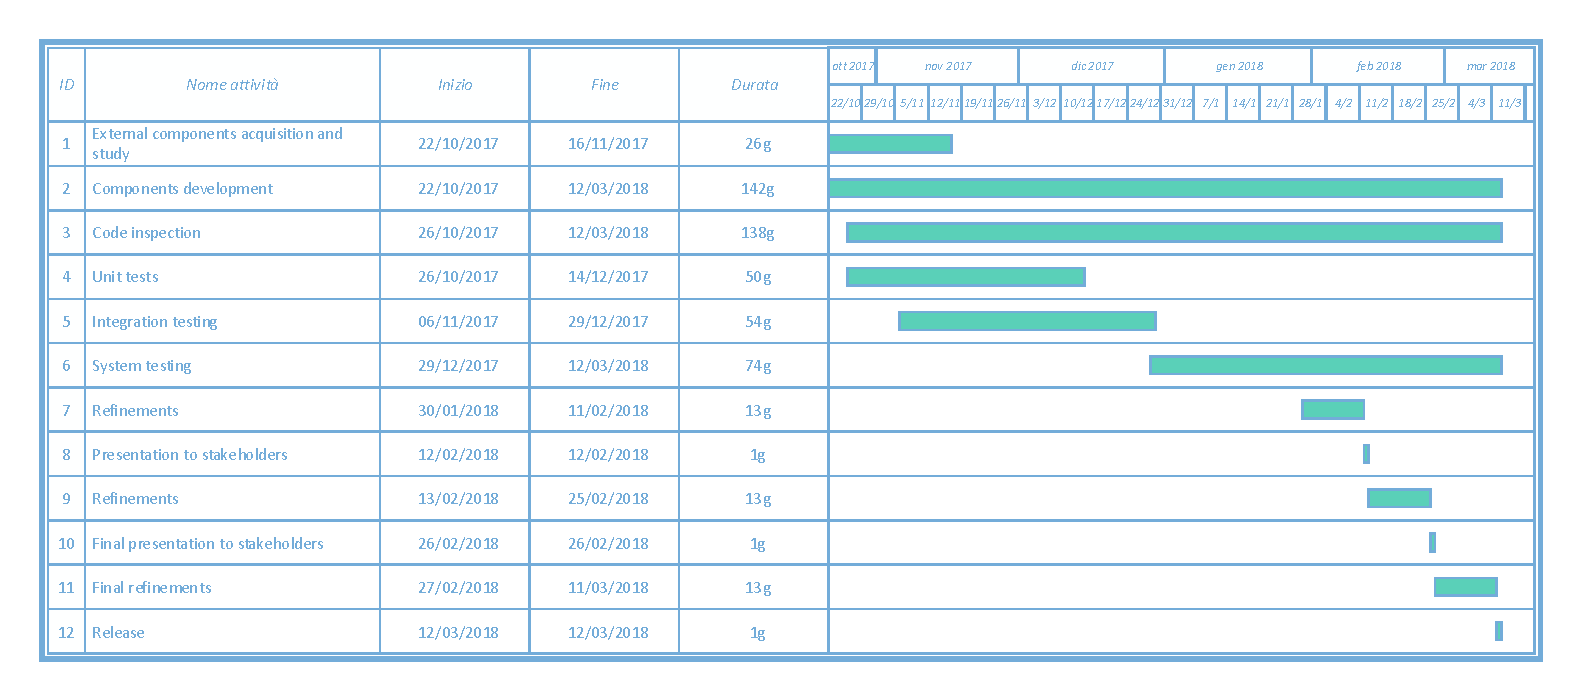
\includegraphics[scale=0.725]{./Images/6-SecondRelease18.pdf} 
		\end{figure}
		\end{landscape}
		\begin{landscape}
	\subsection{Third release}
		\begin{figure}[H]
			\centering
			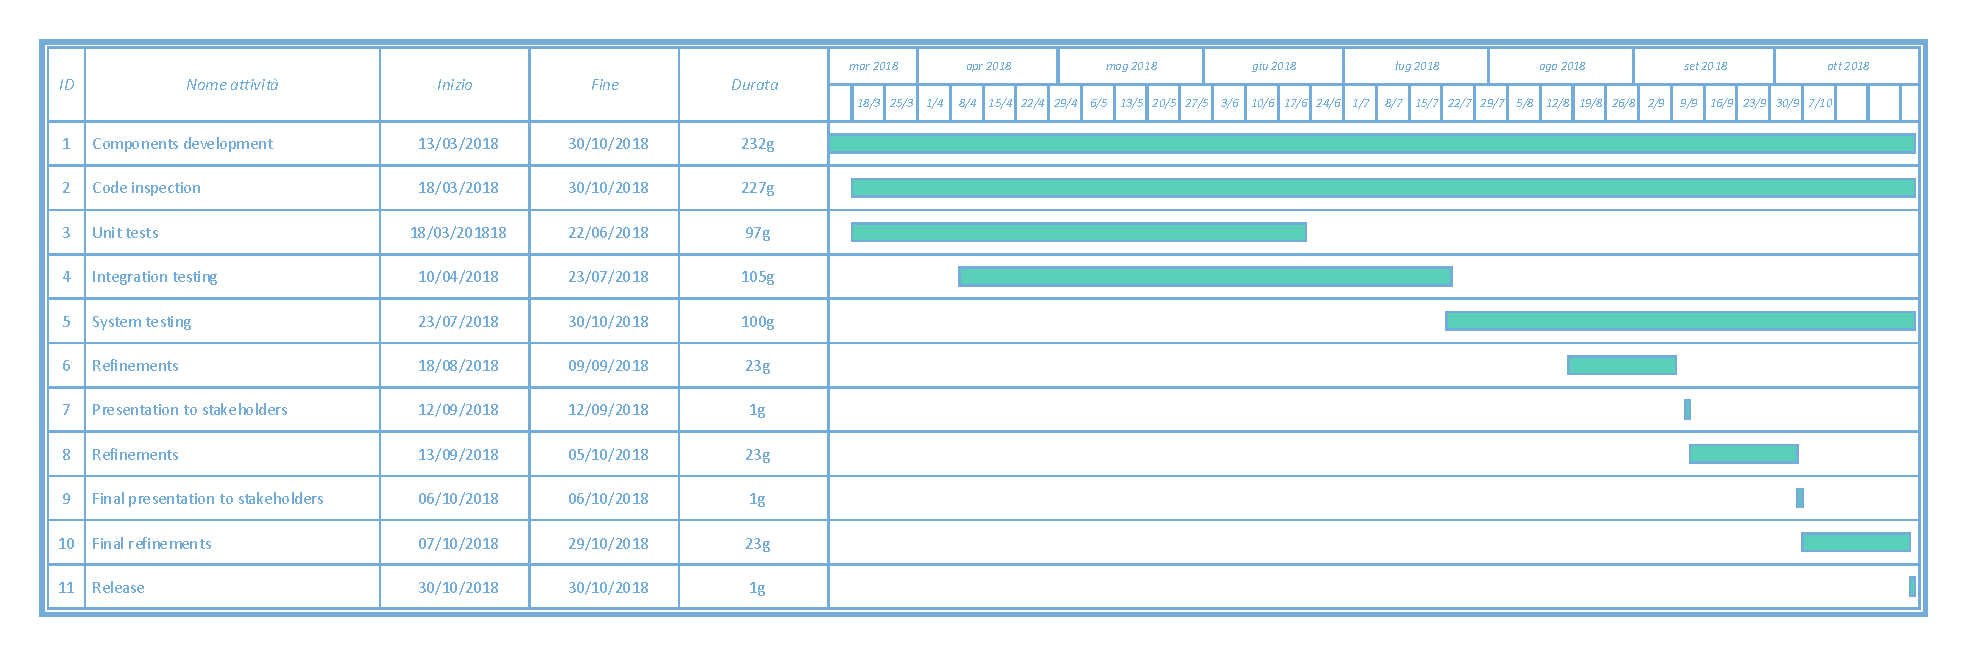
\includegraphics[scale=0.55]{./Images/7-ThirdRelease18.pdf} 
		\end{figure}
		\end{landscape}

\section{Resource allocation}
In  the early analysis and design part of the project we worked together on the various tasks in order to keep a shared view of the product. On the other hand we need additional people to develop the project by deadlines, this requires a form of task assignment to different team members.
\par We adopt a hierarchical approach to accomplish tasks' assignment which consist in people being subdivided into 2 teams, lead by one of the original member. The team leader is assigned an area of the project, and assign tasks to team members. One of the original project member act as project manager, and daily meets with the team leaders, keeping a global perspective on the project.
\par The teams and areas we identified are:
\begin{itemize}
	\item \textbf{Project manager}
	\item{ \textbf{Developers team 1}: Code implementation \\
	 (team leader + 3 members)}
	\item{\textbf{Developers team 2}: Testing\\
	 (team leader + 2 members)}
\end{itemize}
		
\section{Risk management}

	We are going to summarize in tabular format the main risks we think can threat the project and the corresponding mitigating actions we planned.
	We adopt a proactive strategy against most serious risks related to business and a reactive strategy (for which we have allocated additional time in project schedule) for unpredictable threats.
	
	\subsection{Business risks}
	Can jeopardize the entire project and menace the business viability of the project.

	\begin{table}[H]
		\centering
		\begin{tabular}{ p{7cm} c c }
		\textbf{Risk} & \textbf{Probability} & \textbf{Impact} \\ \hline \\
		Due to the high number of competitors in the car sharing panorama, the product can not be noticed if not properly advertised & High & Catastrophical \\ \\
		Unintuitive user interface or wrong set of functionalities drastically reduce the user's adoption of the service & Medium & Catastrophical \\ \\
		Lost of interest in the product by market users / new competitors introduction in the market & Low & Significant \\ \\
		
		Unintuitive user interface reduce the efficiency of the staff & Low & Minor \\ \\
		\end{tabular}
	\end{table}
	
	\begin{table}[H]
		\centering
		\begin{tabular}{ p{6cm} p{6cm} }
		\textbf{Risk} & \textbf{Mitigation plan} \\ \hline \\
		Not properly advertised & Designers, advertisers and sales personnel actively take part to the early stages of UX designing, in order to have a shared vision of the project through all the involved personnel. \\ \\
		Unintuitive user interface / wrong set of functionalities & Surveys and user group to fit the service experience to the average market user. \\ 
		& Analysis of other car-sharing services experience to offer a fast learning curve to their users and emphatize our strength points. \\ \\
		 Lost of interest / new competitors & Occasional in-app quality assessment of the user's service experience in exchange of car sharing credit. \\ \\
		 Low staff enthusiasm / efficiency & Interaction with staff exponent during the early phase of the user interface design through the presentation / assessment of mockups. \\ 
		 & In-house usability test for UI prototypes during the early phases of implementation. \\
		\end{tabular}
	\end{table}
	
	\subsection{Project risks}
	Threaten the project schedule and can increase the project cost.

	\begin{table}[H]
		\centering
		\begin{tabular}{ p{7cm} c c }
		\textbf{Risk} & \textbf{Probability} & \textbf{Impact} \\ \hline \\
		`Goldplating` software features results in a delayed schedule & Low & Significant \\ \\
		Personnel shortfall in proximity of milestones / meeting can delay the release date & High & Minor \\ \\
		\end{tabular}
	\end{table}
	
	\begin{table}[H]
		\centering
		\begin{tabular}{ p{5cm} p{6cm} }
		\textbf{Risk} & \textbf{Mitigation plan} \\ \hline \\ 
		`Goldplating` software features results in a delayed schedule & Planning of 3 features-incremental releases that can be adjusted in feature-richness if schedule problems arise. \\ 		\\
		Personnel shortfall & Introduction of additional time in the schedule between predicted milestone date and milestone release date in order to mitigate personnel absence or for fix eventual problems. 	\\ 
		& Encourage developer motivation through involvement in early analysis phases and in following meetings, thus incentive a shared product vision that lead to better teamwork. \\	
		\end{tabular}
	\end{table}
	
	
	\subsection{Technical risks}
	Threaten the quality and timeliness of the project,  leading to a more difficult implementation.

	\begin{table}[H]
		\centering
		\begin{tabular}{ p{7cm} c c }
		\textbf{Risk} & \textbf{Probability} & \textbf{Impact} \\ \hline \\
		Integration test fails require a redesign of part of the components & Medium & Significant \\  \\
		Unstable external software components / services lead to service partial or full crashes & Low & Significant \\ \\
				\end{tabular}
	\end{table}
	
	\begin{table}[H]
		\centering
		\begin{tabular}{ p{5cm} p{6cm} }
		\textbf{Risk} & \textbf{Mitigation plan} \\ \hline \\
		 Integration test fails  &  Adoption of critical modules test strategy to be able to deal with this kind of issue as soon as possible. \\  \\
		Unstable external software  & Selection of widely adopted services (such as Google Map services). \\
		& Exploration / planning of possible external services' alternatives in case of downtime or discontinuation of those services. \\
		\end{tabular}
	\end{table}
	
	
	

\pagebreak
\section{Effort Spent}

\begin{itemize}
		\item Alessandro Erba $\approx$ 14h
		\item Filippo Leveni 	$\approx$ 14h
		\item Luca Lodi $\approx$ 14h
	\end{itemize}

























\end{document}